\documentclass[12pt]{article}
\usepackage{ctex}
\usepackage[margin=1in]{geometry}		% For setting margins
\usepackage{amsmath}				% For Math
\allowdisplaybreaks  				% 允许跨页显示多行公式
\usepackage{fancyhdr}				% For fancy header/footer
\usepackage{graphicx}				% For including figure/image
\usepackage{lipsum}  % 使用 lipsum 包生成假文(Lorem Ipsum)

%%%%%%%%%%%%%%%%%%%%%%
%公式转跳相关  \eqref{eq:1}
\usepackage{hyperref}     % 支持点击跳转
\usepackage{cleveref}     % (可选)增强引用显示效果
%%%%%%%%%%%%%%%%%%%%%%

%%%%%%%%%%%%%%%%%%%%%%
%绘图
\usepackage{tikz}
\usepackage{pgfplots}
\pgfplotsset{compat=1.18} % 你可以根据你的pgfplots版本调整此设置


%%%%%%%%%%%%%%%%%%%%%%
%方框相关
\usepackage{tcolorbox}  % 创建方框
% 加载列表库,支持多页方框
\tcbuselibrary{listingsutf8}
\tcbuselibrary{breakable} % 确保启用breakable库
%%%%%%%%%%%%%%%%%%%%%%

% 额外设置
\numberwithin{equation}{section}  % 设置公式按section编号
\numberwithin{figure}{section}  % 设置图表按节编号

%%%%%%%%%%%%%%%%%%%%%%
% Set up fancy header/footer
\pagestyle{fancy}
\fancyhead[LO,L]{Yachen Li}
\fancyhead[CO,C]{Lecture Note}
\fancyhead[RO,R]{\today}
\fancyfoot[LO,L]{}
\fancyfoot[CO,C]{\thepage}
\fancyfoot[RO,R]{}
\renewcommand{\headrulewidth}{0.4pt}
\renewcommand{\footrulewidth}{0.4pt}
%%%%%%%%%%%%%%%%%%%%%%


%%%%%%%%%%%%%%%%%%%%%%
% 添加标题
\title{Doppler-free laser spectroscopy}  % 你的标题
\author{李亚宸}  % 作者
\date{\today}  % 日期,自动使用当前日期
%%%%%%%%%%%%%%%%%%%%%%


\begin{document}

\maketitle  % 在文档中显示标题、作者和日期
\thispagestyle{fancy}  % 强制第一页显示页眉和页脚

\section{Doppler broadening of spectral lines}
在实验室参考系中辐射的角频率 $\omega$ 和在以速度 $v$ 运动的相对参考系中看到的该辐射的角频率之间的关系为
\begin{align}\label{eq:8.1}
	\omega' = \omega - kv 
\end{align}
其中该辐射的波失 $ k=\omega /c=2\pi /\lambda  $。沿 $ \mathbf{k} $ 方向的速度分量将贡献一阶多普勒效应,并且我们假设 $ \mathbf{k}\cdot \mathbf{v}=kv $。

\begin{figure}[!h] 
	\begin{centering}
		\includegraphics[keepaspectratio = true, width = 3in]{images/8-1.png}
		\caption{观测辐射频率时的多普勒效应。}
	\end{centering}
\end{figure}

在这里我们考虑一团原子吸收辐射时的多普勒效应。假设每个原子在它自己的相对参考系中只吸收频率为 $ \omega _0 $ 的辐射,即当 $ \omega'=\omega _0 $ 时。于是以速度 $ v $ 运动的原子将会在 $ \delta =\omega -\omega _0=kv $ 时才吸收辐射,或者等效地
\begin{align}\label{eq:8.2}
	\frac{\delta}{\omega_0} = \frac{v}{c}
\end{align}

\begin{tcolorbox}[colback=red!3, colframe=red!60!black, title=注释, breakable]
	由
	\begin{align}
		\delta &=\omega -\omega _0=kc-\omega _0=kv \notag \\
		&\Longrightarrow \omega _0=k\left( c-v \right) \tag{1}
	\end{align}
	有
	\begin{align}
		\frac{\delta}{\omega _0}=\frac{kv}{k\left( c-v \right)}\simeq \frac{v}
		{c}\tag{2}
	\end{align}
\end{tcolorbox}

在一团原子气体中,速度范围在 $ v $ 到 $ v + dv $ 的原子所占的比例为
\begin{align}\label{eq:8.3}
	f(v) \, \mathrm{d}v = \sqrt{\frac{M}{\pi 2 k_B T}} \exp \left( -\frac{M v^2}
	{2 k_B T} \right) \mathrm{d}v \equiv \frac{1}{u \sqrt{\pi}} \exp \left( -
	\frac{v^2}{u^2} \right) \mathrm{d}v
\end{align}

\begin{tcolorbox}[colback=red!3, colframe=red!60!black, title=注释, breakable]
	\centering
	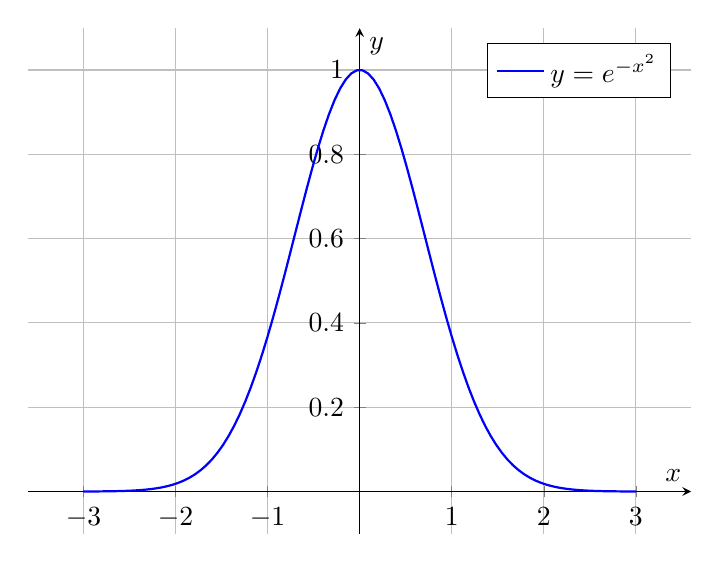
\begin{tikzpicture}
    \begin{axis}[
        axis lines = middle,
        xlabel = $x$,
        ylabel = $y$,
        domain = -3:3,
        samples = 100,
        grid = both,
        width = 10cm, height = 8cm,
        enlargelimits,
        legend pos = north east,
    ]
    \addplot[blue, thick] {exp(-x^2)};
    \addlegendentry{$y = e^{-x^2}$}
    \end{axis}
	\end{tikzpicture}

	\centering
	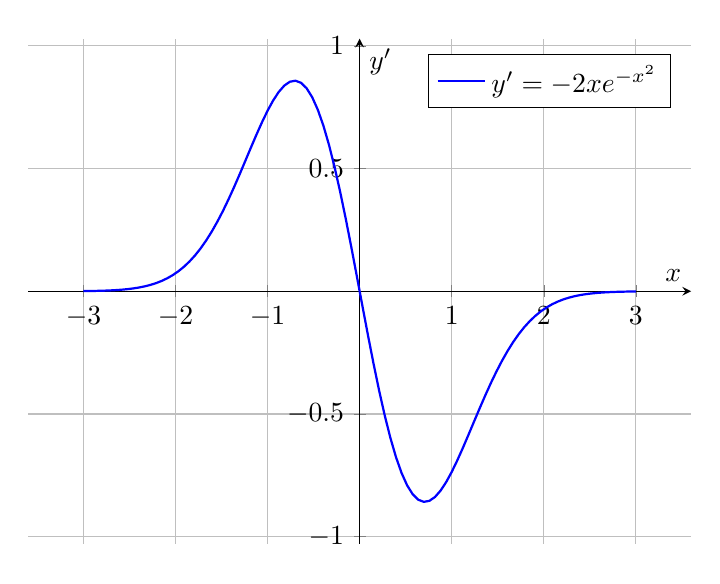
\begin{tikzpicture}
    \begin{axis}[
        axis lines = middle,
        xlabel = $x$,
        ylabel = $y'$,
        domain = -3:3,
        samples = 100,
        grid = both,
        width = 10cm, height = 8cm,
        enlargelimits,
        legend pos = north east,
    ]
    \addplot[blue, thick] {-2*x*e^(-x^2)};
    \addlegendentry{$ y'=-2xe^{-x^2} $}
    \end{axis}
	\end{tikzpicture}
\end{tcolorbox}

其中 $ u = \sqrt{2k_B T / M} $ 是最概然速度。利用式 \ref{eq:8.2} 将速度代换为频率,我们可以发现吸收函数具有高斯线形:
\begin{align}\label{eq:8.4}
	g_D (\omega) = \frac{c}{u \omega_0 \sqrt{\pi}} \exp \left\{ -\frac{c^2}{u^2} 
	\left( \frac{\omega - \omega_0}{\omega_0} \right)^2 \right\}
\end{align}

\begin{tcolorbox}[colback=red!3, colframe=red!60!black, title=注释, breakable]
	\begin{align}
		f\left( v \right) \text{d}v &=\frac{1}{u\sqrt{\pi}}\exp \left( -
		\frac{v^2}{u^2} \right) \text{d}v \notag \\
		&=\frac{1}{u\sqrt{\pi}}\exp \left[ -\frac{1}{u^2}\left( c\frac{\omega -
		\omega _0}{\omega _0} \right) ^2 \right] \text{d}\left( c\frac{\omega -
		\omega _0}{\omega _0} \right)  \notag \\
		&=\frac{1}{u\sqrt{\pi}}\exp \left[ -\frac{c^2}{u^2}\left( \frac{\omega -
		\omega _0}{\omega _0} \right) ^2 \right] \frac{c}{\omega 
		_0}\text{d}\omega  \notag \\
		&=\frac{c}{u\omega _0\sqrt{\pi}}\exp \left[ -\frac{c^2}{u^2}\left( 
		\frac{\omega -\omega _0}{\omega _0} \right) ^2 \right] \text{d}\omega 
		\tag{1}
	\end{align}
\end{tcolorbox}

该函数的最大值取在 $ \omega =\omega _0 $ 处,并在 $ \omega -\omega _0=\delta _{1/2} $ 处取得最大值的一半,其中
\begin{align}\label{eq:8.5}
	\left( \frac{c \delta_{1/2}}{u \omega_0} \right)^2 = \ln 2
\end{align}

\begin{tcolorbox}[colback=red!3, colframe=red!60!black, title=注释, breakable]
	\begin{align}
		\frac{1}{2}g_{D\max}\left( \omega \right) &=\frac{c}{2u\omega 
		_0\sqrt{\pi}}=\frac{c}{u\omega _0\sqrt{\pi}}\exp \left\{ -\frac{c^2}
		{u^2}\left( \frac{\omega -\omega _0}{\omega _0} \right) ^2 \right\}
		\notag \\
		&\Rightarrow \frac{1}{2}=\exp \left\{ -\frac{c^2}{u^2}\left( 
		\frac{\omega -\omega _0}{\omega _0} \right) ^2 \right\}  \notag \\
		&\Longrightarrow \ln \frac{1}{2}=-\ln 2=-\frac{c^2}{u^2}\left( 
		\frac{\omega -\omega _0}{\omega _0} \right) ^2 \notag \\
		&\Longrightarrow \ln 2=\left( \frac{c\delta}{u\omega _0} \right) ^2 
		\notag \\
		&\Longrightarrow \delta =\omega -\omega _0=\pm \omega _0\sqrt{\ln 
		2}\frac{u}{c} \tag{1}
	\end{align}
\end{tcolorbox}

多普勒增宽线形的半高全宽为 $ \Delta \omega _{\text{D}}=2\delta _{1/2} $
\begin{align}\label{eq:8.6}
	\frac{\Delta \omega_D}{\omega_0} = 2 \sqrt{\ln 2} \frac{u}{c} \simeq 1.7 
	\frac{u}{c}
\end{align}

多普勒效应对原子气体吸收辐射的影响是非均匀增宽的一个例子。由于频率失谐依赖于原子的速度,各个原子由于具有不同速度而和辐射的相互作用是不同的。相比之下,由激发态自发辐射造成的辐射增宽为气体中所有原子提供了相同的自然线宽,这是一种均匀增宽机制。

\section{Saturated absorption spectroscopy}
我们在上一节通过假设原子在自身参考系中只在 $ \omega_0 $ 处吸收辐射,推导出了多普勒增宽的线形。但实际上,原子可以在一定频率范围内吸收辐射,这个频率范围由跃迁的均匀线宽给出。在这一节,我们将重新审视吸收单色辐射的过程,其中既包括均匀增宽,也包括由原子运动产生的非均匀增宽,这将很自然地引出对饱和吸收光谱的讨论。

\begin{figure}[!h] 
	\begin{centering}
		\includegraphics[keepaspectratio = true, width = 3in]{images/7-4.png}
		\caption{在厚度为Δz的薄片中分布的数密度为N的原子,会吸收入射光束强度的NσΔz部分,其中σ定义为吸收截面。NΔz是每单位面积的原子数,σ表示每个原子呈现的“目标”面积。我们假设可以忽略目标原子的运动,并且假设下一层(厚度为δz)的原子不能“躲”在这些原子后面。}
		\label{fig:7.4}
	\end{centering}
\end{figure}
我们考虑一束强度为 $ I\left( \omega \right)  $ 的激光穿过原子样品,如图 \ref{fig:7.4} 所示。运动速度在 $ v $ 到 $ v+\text{d}v $ 范围内的原子将会在自身参考系中看到有效辐射频率 $ \omega -kv $,这些原子的吸收截面为 $ \sigma \left( \omega -kv \right)  $,其中吸收截面定义为
\begin{align}\label{eq:7.76}
	\sigma(\omega) = 3 \times \frac{\pi^2 c^2}{\omega_0^2} A_{21} g_H(\omega)
\end{align}

\begin{align}\label{eq:8.11}
	\kappa(\omega) &= \int N(v) \sigma(\omega - kv) \, \mathrm{d}v \notag \\
	&= \frac{g_2}{g_1} \frac{\pi^2 c^2}{\omega_0^2} A_{21} \times \int N(v) g_H(\omega - kv) \, \mathrm{d}v \notag \\
	&= \frac{g_2}{g_1} \frac{\pi^2 c^2}{\omega_0^2} A_{21} \times N \int f(v) \frac{\Gamma/(2\pi)}{(\omega - \omega_0 - kv)^2 + \Gamma^2/4} \, \mathrm{d}v
\end{align}



\noindent \textit{A uniformly charged dielectric gel having charge density $\rho_v = \rho_o$ and dielectric constant of $\epsilon_r = 2$ is enclosed inside a dielectric shell with dielectric constant of $\epsilon_r = 5$ as shown in the figure. The dielectric shell is surrounded by free space ($\epsilon_r = 1$). Determine E, $\Phi$, D, P in all regions.}
中国科学技术大学

\begin{figure}[!h] 
	\begin{centering}
		\includegraphics[keepaspectratio = true, width = 2in]{image.PNG}
		\caption{Given scenario.}
	\end{centering}
\end{figure}

\noindent In this problem we can consider there to be 3 regions, (1)~$r < a$, (2)~$a \leq r < b$, and (3)~$r \geq b$. For finding the electric flux density Gauss's Law provides the most straight forward solution. Then, using the constitutive relation between electric flux density and electric field, $\vec{E}$ can be found. Thereafter $\vec{P}$ and $\Phi$ are directly related to $\vec{E}$.\\
\\

\section{第二节}
Gauss's Law provides the most straight forward solution Gauss's Law provides the most straight forward solution Gauss's Law provides the most straight forward solution Gauss's Law provides the most straight forward solution Gauss's Law provides the most straight forward solution Gauss's Law provides the most straight forward solution Gauss's Law provides the most straight forward solution Gauss's Law provides the most straight forward solution Gauss's Law provides the most straight forward solution Gauss's Law provides the most straight forward solution Gauss's Law provides the most straight forward solution 

\begin{tcolorbox}[colback=red!3, colframe=red!60!black, title=注释, breakable]
	\begin{align}
		F=ma \notag
	\end{align}
	\begin{align}
		E=mc^2 \notag
	\end{align}
	Gauss's Law provides the most straight forward solution Gauss's Law provides the most straight forward solution Gauss's Law provides the most straight forward solution Gauss's Law provides the most straight forward solution \cite{bib1}
\end{tcolorbox}



%%%%%%%%%%%%%%%%%%%%%%
%参考文献
\begin{thebibliography}{2} % 这里的数字是指参考文献总数目,需要根据实际情况进行修改
    \bibitem{bib1} Foot C J. Atomic physics[M]. Oxford University Press, 2005.
\end{thebibliography}
%%%%%%%%%%%%%%%%%%%%%%
		


\end{document}